\chapter{Estado del arte}\label{Chapter2} 
\section{Conservación de procedimiento científicos}

Distintas áreas de la ciencia han adoptado técnicas y herramientas para conservar el procedimiento. Por ejemplo, investigadores en bio-informática ha incorporado los workflows para distintos análisis:  Doblamiento de proteínas \cite{craddock2006science}, secuencias de DNA y RNA \cite{blankenberg2010galaxy,giardine2005galaxy} y la detección de ondas gravitacionales \cite{deelman2004pegasus}.
Los workflows científicos son métodos que permiten representar un conjunto de pasos computacionales. Estos pasos pueden ser la obtención de los datos de entrada, transformaciones o generación de los resultados.
La representación de los workflow se construye en un lenguaje abstracto para simplificar la complejidad. El conjunto de pasos se pueden representar como grafos sin ciclos y dirigidos, donde cada paso computacional es representado por un nodo y las dependencias entre los pasos son representado por los arcos.
El uso de sistemas de manejo de workflows científicos \textit{Scientific Workflow management Systems (WMS)} permiten diseñar abstractamente, ejecutar y compartir el procedimiento científicos. 

Dado que los workflows formalmente describen la secuencia de tareas computacionales y administración de datos, es fácil encontrar el camino de los datos producidos.
Un científico podría ver el workflow y los datos, seguir los pasos y llegar al mismo resultado. En otras palabras, la representación del workflow facilita la creación y administración de la computación y además construye una base en la cual los resultados pueden ser validados y compartidos.

%\todo{Colocar citas de los estudios} 
%Sin embargo, múltiples estudios han mostrado las dificultades reproducir los resultados de los experimentos.

%todo: ampliar estos


%Como se menciono, la mayoría de las propuestas de reproducibilidad de ambientes en las ciencias de computación se han enfocado en los datos, el código y la descripción de workflow pero ha dejando de lado los recursos computacionales y componentes de software. Siendo un recurso esencial para reproducir el experimento

%De acuerdo a \cite{king1995replication}, en orden de reproducir o replicar un artefacto digital es necesario manejar su conservación y para alcanzar esta conservación se debe garantizar que: existe la suficiente información con la cual se pueda entender, evaluar y construir un trabajo anterior sin información adicional del autor. 

%Uno de los trabajos que se ha enfocado en conservar los recursos de un ambiente computacional es \cite{santana2017reproducibility}. Donde los autores han identificado dos enfoques para conservar un ambiente científico. Conversación física: donde el objeto real es conservado dada la relevancia y la dificultada de obtener una replica y  Conversación lógica: donde los objetos son descriptos en una manera que un experimento similar puede ser obtenido en un futuro experimento.


\subsection{Sistemas de administración de workflows}

Cómo se menciono anteriormente, los workflows científicos permiten a los usuarios expresar fácilmente tareas computacionales de varios pasos, por ejemplo, recuperar datos de un instrumento o una base de datos, dar un formato a los datos y ejecutar un análisis. 
Un workflow científico describe las dependencias entre las tareas y la mayoría de los WMSs utiliza la descripción de un gráfico acíclico dirigido (DAG), donde los nodos son tareas y los bordes denotan las dependencias de las tareas.
Una propiedad que define un workflow científico es que gestiona el flujo de datos. Es por ello, que las tareas en un  workflow científico varían ampliamente según las necesidades del autor, los tipos pueden ser tanto como tareas cortas en serie o tareas paralelas muy grandes (e.g, utilizando Message Passing Interface - MPI) rodeadas de un gran número de pequeñas tareas en serie utilizadas para el pre y post procesamiento.
La interpretación y ejecución de los workflows son manejados por un sistema de manejo de workflows (WMS) que administra la ejecución de la aplicación en la infraestructura. 
Un WMS puede ser considerado como una capa intermedia necesaria para la abstracción y orquestación de procedimiento científico. A continuación se describen algunos de los WMSs más populares.

\subsection{Galaxy}	
Galaxy \cite{goecks2010galaxy} es un sistema de gestión de almacenes basado en la web que tiene como objetivo llevar las capacidades de análisis de datos computacionales a usuarios no expertos en el campo de las ciencias biológicas. Los principales objetivos del marco de trabajo de Galaxy son la accesibilidad a las capacidades computacionales biológicas y la reproducibilidad del resultado del análisis mediante el seguimiento de la información relacionada con cada paso del proceso. 

\subsection{Taverna}	
Taverna \cite{DBLP:journals/bioinformatics/OinnAFMSGCGPWL04} es un WMS basado en servicios web, ya que todos los componentes del flujo de trabajo deben implementarse cómo servicios web (ya sea localmente o utilizando un servicio remoto disponible). 
Taverna permite a un científico que tiene una experiencia limitada en informática, recursos técnicos y soporte limitados, construir análisis altamente complejos sobre datos y recursos computacionales que son tanto públicos como privados, utilizando cualquier sistema operativo.
Además, Taverna provee integraciones con myExperiment~\cite{goble2010myexperiment} y BioCatalogue~\cite{bhagat2010biocatalogue} y provee servicios para ejecutar código Java local, uso de lenguaje R \footnote{\url{https://www.r-project.org/}} , scripts XPath o servicios de importación de hojas de cálculo.

\subsection{Pegasus}
Pegasus\cite{deelman2004pegasus} abarca un conjunto de tecnologías que ayudan a que las aplicaciones basadas en workflow se ejecuten en diferentes entornos, incluyendo escritorios, clusters de campus, grillas y nubes. Pegasus tiende un puente entre el dominio científico y el entorno de ejecución mediante la asignación automática de descripciones de workflow de alto nivel a recursos distribuidos. 
Siendo capaz gestionar flujos de trabajo compuestos por millones de tareas, registrando datos sobre la ejecución y resultados intermedios.
En Pegasus, los flujos de trabajo se describen como flujos de trabajo abstractos, que no contienen información de recursos, o las ubicaciones físicas de datos y ejecutables.

\subsection{WINGS}  
 
WINGS \cite{DBLP:journals/expert/GilRKGGMD11} es un sistema de workflow semántico que ayuda a los científicos en el diseño de experimentos computacionales.
La diferenciación de WINGS respecto a otros WMSs es que incorporan restricciones semánticas sobre conjuntos de datos y componentes de flujo de trabajo, a partir de esas restricciones éstos se crean y validan para generar los resultados.  
WINGS puede considerarse como una herramienta de diseño de alto nivel y orientada a los dominios, cuyos workflows pueden ejecutarse posteriormente en diferentes motores de WMSs, como Pegasus~\cite{deelman2004pegasus} o Apache OODT \footnote{\url{http://oodt.apache.org/}}.

%todo: mejorar esto
\subsection{dispel4py}
dispel4py \cite{DBLP:conf/eScience/FilgueiraKAKSS15}  es una biblioteca Python para describir flujos de trabajo. 
 Describe flujos de trabajo abstractos para aplicaciones intensivas en datos, que luego se traducen y ejecutan en plataformas distribuidas (por ejemplo, Apache Storm, clusters MPI, etc.).
Uno de los objetivos es que los usuarios se centren en sus métodos científicos, evitando que se distraigan en los detalles y manteniendo la flexibilidad sobre la infraestructura informática que utilizan. 


\section{Conservación de equipamiento}
Comúnmente en otras disciplinas que realizan estudios \emph{in-vivo}, el equipamiento no es un problema a resolver dado que los recursos utilizados son conocidos, no-variables y estándares. Por ejemplo en la biología ó quimica, la utilización de probetas, microscopios u otros elementos físicos. 
Consecuentemente, los investigadores pueden nombrarlos e identificarlos de forma manual en los procedimientos de sus cuadernos de laboratorio. Lo que permite que otro investigador conozca cuáles fueron las herramientas utilizadas en el experimento.
Aunque existen excepciones, donde ciertos recursos son materiales que son utilizados en los procedimientos. En estos casos, los investigadores deben describir los materiales incluyendo información como marcas, composición y otros. 
Otro caso es en la astronomía, donde se utilizan recursos de alta tecnología, donde también es necesario documentar las características de hardware y configuraciones utilizadas en el proceso experimental. 
En las ciencias de la computación sucede un caso similar, dado que los recursos computacionales son una componente requerida en la ejecución del sistema. 
Es por ello, que esta comunidad no puede ser la excepción respecto a la descripción de los recursos. Por lo tanto, los autores deben documentar computadores, clusters, servicios web, componentes de software, etc., en el contexto de sus experimentos.

Diversos trabajos han estudiado el estado actual de la reproducibilidad de estudios \emph{in-silico}, en \cite{DBLP:conf/eScience/ZhaoGBKGGHRRG12} se estudia el factor de decaimiento de un conjunto workflows científicos almacenado en myExperiment \footnote{\url{https://www.myexperiment.org/home}} que fueron diseñados para el WMS Taverna \cite{DBLP:journals/bioinformatics/OinnAFMSGCGPWL04} del área de biología. Para ello, los autores utilizaron cuatro conjuntos de paquetes de workflows y clasificaron el decaimiento de los workflows en cuatro categorías: recursos de terceros volátiles, datos de ejemplos faltantes, ambiente de ejecución faltante y descripciones insuficientes sobre los workflow. El estudio muestra que casi el 80\% de workflows fallan al ser reproducidos, con un 12\% de esos fallos debido al ambiente de ejecución faltante y 50\% recursos de terceros volátiles. Estas dos últimas categorías están asociadas a la conservación del ambiente computacional del experimento.
En \cite{DBLP:conf/ipres/MatthewsCWJBS09}, los autores describen un procedimiento para preservar el software, argumentando que el software es frágil a los cambios de ambiente ya sea hardware, sistema operativo, versiones de las dependencias y configuración. Los autores afirman que el software no puede ser preservado con la metodología de sólo mantener su código binario ejecutable recomendando el empaquetamiento de software. También, introducen el concepto de adecuación de la preservación, una métrica para medir si la preservación de conjunto de funcionalidades de componente de software luego de un proceso reproducción.

De la misma manera, editoriales se ha enfocado en intentar resolver los desafíos en la publicación de trabajos científicos. Por ejemplo, Elsevier formó el \textit{Executable Paper Grand Challenge} para abordar la dificultad de reproducibilidad de los resultados en las ciencias de la computación, ellos  argumentan que los bloques vitales y necesarios de información para replicar los resultados -por ejemplo, software, código, grandes conjuntos de datos- no suelen estar disponibles en el contexto de una publicación académica. 
Es por ello que \textit{Executable Paper Grand Challenge} creó una oportunidad para que los científicos diseñen soluciones que capturen esta información y proporcionen una plataforma para que estos datos puedan ser verificados y manipulados. 
En 2011, \cite{DBLP:journals/procedia/BrammerCMW11} se argumenta que el documento de investigación en su estado actual ya no es suficiente para reproducir, validar o revisar completamente los resultados y conclusiones experimentales de un documento. Esto impide el progreso científico. 
Para remediar estas preocupaciones, presentan Paper Mâché, un nuevo sistema para crear documentos de investigación dinámicos y ejecutables. La principal novedad de Paper Mâché es el uso de máquinas virtuales, que permite a los lectores y revisores ver e interactuar fácilmente con un documento y poder reproducir los principales resultados experimentales.
En la misma línea, CernVM~\footnote{\url{https://cernvm.cern.ch/}}~\cite{buncic2010cernvm} propuso la utilización de máquinas virtuales para resolver problemas de reproducibilidad en la ciencia. CernVM es un sistema para el uso de máquina virtuales capaz de ejecutar aplicaciones físicas de los experimentos relacionados al \textit{Large Hadron Collider} (LHC) en el \textit{European Organization for Nuclear Research} (CERN). Su objetivo es proporcionar un entorno completo y portátil para desarrollar y ejecutar el análisis de datos generados por el LHC en cualquier ordenador del usuario final (portátil, de mesa), así como en la red, independientemente de las plataformas de sistemas operativos (Linux, Windows, MacOS). 
CernVM logra lo anterior haciendo so de técnicas de virtualización que permite separar los recursos de computación desde la infraestructura subyacente.

Algunos autores han expuesto la necesidad de capturar y preservar el entorno de ejecución del experimento, proporcionando herramientas para analizar y empaquetar los recursos involucrados en él.
ReproZip \cite{DBLP:conf/tapp/ChirigatiSF13} busca captar el conocimiento sobre una infraestructura e intentar reproducirla en un nuevo entorno. Esta herramienta lee los componentes de infraestructura involucrados en la ejecución (archivos, variables de entorno, etc.) y almacena esta información en una base de datos MongoDB \footnote{\url{https://www.mongodb.com/es}}. 
A continuación se recogen y empaquetan los elementos descritos. Luego, el sistema debe desempaquetar los elementos en otra máquina para reproducir el experimento. 
Sin embargo, este tipo de enfoque que empaqueta los componentes físicos de una infraestructura determinada presenta una limitación en la práctica, debido que los paquetes deben ser ejecutado en una máquina destino similar.
Otro ejemplo es TOSCA (Topology and Orchestration Specification for Cloud Applications), TOSCA es un ejemplo de las soluciones que han definido sintaxis para describir la ejecución de los ambientes computacionales. TOSCA es un lenguaje de código abierto utilizado para describir las relaciones y dependencias entre servicios y aplicaciones que residen en una plataforma de computación. TOSCA puede describir un servicio de computación en nube y sus componentes y documentar la forma en que están organizados y el proceso de orquestación necesario para utilizar o modificar dichos componentes y servicios. Esto proporciona a los administradores una forma común de gestionar aplicaciones y servicios en la nube, de modo que esas aplicaciones y servicios puedan ser portátiles a través de las diferentes plataformas de los proveedores de Cloud Computing. 
Otro esfuerzo importante relacionado a nuestro trabajo incluye la descripción de los ambientes computaciones utilizando ontologías es TIMBUS. El proyecto se focaliza en preservar procesos de negocios y su infraestructura computacional. 
Para ello, propusieron un extractor para extraer y anotar los componentes de Software y Hardware, éstas anotaciones son almacenadas según un conjunto de ontologías con el objetivo de gestionar la preservación y ejecución de los procesos de negocio. 
Sin embargo, el enfoque extractor del Proyecto Timbus no es adecuado para ser utilizado en cualquier sistema ya que aumenta la complejidad del ambiente y exige la instalación de componentes de terceros dentro del ambiente, lo cual provoca ruido. 
Además, exige ejecutar el ambiente computacional lo cual conlleva altos costos computacionales, disminución en la escalabilidad del sistema y creación de brechas de seguridad. 

En el enfoque de describir los recursos computacionales, los autores en \cite{santana2017reproducibility} identificaron dos enfoques para conservar el  ambiente computacional de un experimento científico: la conservación física, donde los objetos de investigación dentro del experimento se conservan en un entorno virtual; y la conservación lógica, donde las principales capacidades de los recursos en el entorno se describen utilizando vocabularios semánticos para permitir al investigador reproducir un entorno equivalente.
Para ello, definieron un proceso para documentar la aplicación del workflow y su sistema de gestión relacionado, así como sus dependencias.
Además, los autores propusieron \textit{The Workflow Infrastructure Conservation Using Semantics ontology} (WICUS). WICUS es una red de ontologías OWL2 (Web Ontology Language) que implementan la conceptualización de los principales dominios de una infraestructura computacional. Como: Hardware, Software, Workflow y Recursos Informáticos. 
Los autores argumentan su importancia de su trabajo debido que a que los workflows científicos requieren un conjunto de componentes de software, y los investigadores deben saber cómo desplegar esta pila de software para lograr un entorno equivalente.
Sin embargo, este proceso se realiza de forma de manual, dejando mucho trabajo a los científicos.
Además, los autores afirman que la conservación de los ambientes computacionales comúnmente se logra utilizando un enfoque físico dado que la conservación física permite compartir fácilmente un ambiente computacional con otros investigadores y ellos pueden reproducir el experimento utilizando en el mismo ambiente. 
Sin embargo, los esfuerzos necesarios para mantener la infraestructura son altos dado el uso del almacenamiento y que no hay garantías que no sufran un proceso de decaimiento \cite{DBLP:journals/fgcs/DeelmanVJRCMMCS15}.  
Consecuentemente, la mayoría de los trabajos dejan fuera la conservación física del entorno informático del workflow. Pese a que la conservación lógica y física son deseadas para lograr la reproducibilidad del experimento.

En diversos trabajos ~\cite{DBLP:journals/bioinformatics/LeprevostGARUBV17, Beaulieu2017, Boettiger:2015:IDR:2723872.2723882, aranguren2015enhanced} se ha propuesto la utilización de Docker como un reemplazo al uso de máquinas virtuales como ambiente computacionales científicos, los trabajos argumentan que Docker presenta beneficios de portabilidad, documentación precisa de la instalación y configuración, manejo de control de versiones de las imágenes y fácil adopción por desarrolladores. 
Un ejemplo de uso de Docker para la reproducibilidad es Bio Containers \cite{DBLP:journals/bioinformatics/LeprevostGARUBV17}. Bio Containers es un framework de código abierto y orientado a la comunidad que proporciona entornos ejecutables independientes de la plataforma para el software de informática.
Bio Containers permite a los laboratorios instalar fácilmente software de bio-informática, mantener múltiples versiones del mismo software y combinar herramientas de análisis. 
Para ello, se basan en los populares proyectos de código abierto Docker~\footnote{\url{https://www.docker.com/}}, Singularity~\footnote{\url{https://www.sylabs.io/singularity/}} y rkt~\footnote{\url{https://coreos.com/rkt/}}, que permiten que el software sea instalado y ejecutado bajo un entorno aislado y controlado.
Sin embargo, en \cite{Boettiger:2015:IDR:2723872.2723882,DBLP:conf/semweb/OsorioAV18} los autores exponen que Docker no controla que paquetes instalados en las imágenes y no existe una descripción completa de los componentes de la imagen y consecuente del contenedor.
Por lo tanto, las imágenes Docker funcionan como una caja negra, lo que significa que los usuarios saben cuál es el paquete que se ejecuta dentro del contenedor pero no conocen las versiones o los otros paquetes necesarios para ejecutarlo.

Respecto a la descripción de los componentes de una imagen Docker, en \cite{Shu:2017:SSV:3029806.3029832:DockerHub:Security} analizó más de 300.000 imágenes de Docker almacenadas en el repositorio oficial de Docker. Los autores encontraron que en promedio las imágenes que contiene el Docker Hub (sistema de almacenamiento de imágenes) son más de 180 vulnerabilidades, siendo la raíz de tal cantidad de vulnerabilidades el hecho de que muchas imágenes no han sido actualizadas en varios días y que muchas de estas vulnerabilidades se propagan de imágenes de padres a hijos. Los autores encontraron correlaciones entre las imágenes más influyentes y los paquetes vulnerables mejor clasificados, lo que sugiere que la fuente de esa cantidad de vulnerabilidades era probablemente el resultado de la propagación de un pequeño número de imágenes populares (debido a la falta de actualización de las imágenes principales). Los autores utilizaron el software Clair \footnote{\url{https://github.com/coreos/clair}} de la empresa CoreOS\footnote{\url{https://coreos.com/}}. 
En términos de ingeniería ontológica, los autores en~\cite{huo2015smart} presentan la ontología Smart contenedor que extiende DOLCE~\cite{gangemi2002sweetening} y modela Docker en términos de sus interacciones para desplegar imágenes. Otro trabajo relacionado, ~\cite{tommasini2017representing}  describe cómo usar RDF para representar archivos de construcción de Docker. 

\section{Docker}

Durante los últimos veinte años el uso de tecnologías de virtualización ha aumentado
	rápidamente, esta tecnología permite dividir el sistema de un computador
	en múltiples ambientes virtuales.
Uno de los usos comunes para esta tecnología es la virtualización de 
	servidores en \textit{datacenters}. Con la virtualización de servidores, un
	administrador de sistemas puede crear una o más instancias virtuales, ya sea
	máquinas virtuales (VMs) o contenedores, en un servidor.
Este enfoque hoy se utiliza comúnmente en \textit{datacenters} y también en plataformas de \textit{Cloud} como Amazon EC2~\footnote{\url{https://aws.amazon.com/es/}}, RackSpace~\footnote{\url{https://www.rackspace.com/es}}, Google Cloud~\footnote{\url{https://cloud.google.com/}} y otros \cite{felter2014updated}. 
A partir del crecimiento del uso de la virtualización ha sido necesario la búsqueda de una solución que permita tener un ambiente escalable y seguro. 
Un gran numero de soluciones han nacido en el mercado y se pueden clasificar en dos tipos: \textit{virtualización basada en contenedores} y \textit{virtualización basada en hipervisores}. 
La primera es una virtualización liviana a nivel de software usando el kernel de host para correr múltiples ambientes virtuales. Estos ambientes son nombrados con contenedores (contenedores).
Y hoy en día Linux-VServer, OpenVZ, libcontainer y Linux container (LXC) son
	las principales implementaciones para utilizar contenedores. En la
	figura~\ref{fig:contenedor-arch} se puede observar que la arquitectura de
	de una virtualización basada en contenedores, éstos utilizan el sistema	
	operativo compartido del ambiente virtualizador (host) y por lo tanto no es
	necesario cargar nuevamente el sistema operativo para cada contenedor que se está
	ejecutado.
Desde el punto de vida del sistema operativo del \textit{host}, los procesos del contenedor no son especiales y se tratan como cualquier otro proceso que ejecuta sobre el kernel.
Sin embargo, los contenedores son ambientes aislados y con recursos limitados y estas características se lograr a través de herramientas del Kernel \cite{merkel2014docker}.
	
\begin{figure*}[t]
    \centering
    \begin{subfigure}[b]{0.48\textwidth}
         \centering
    	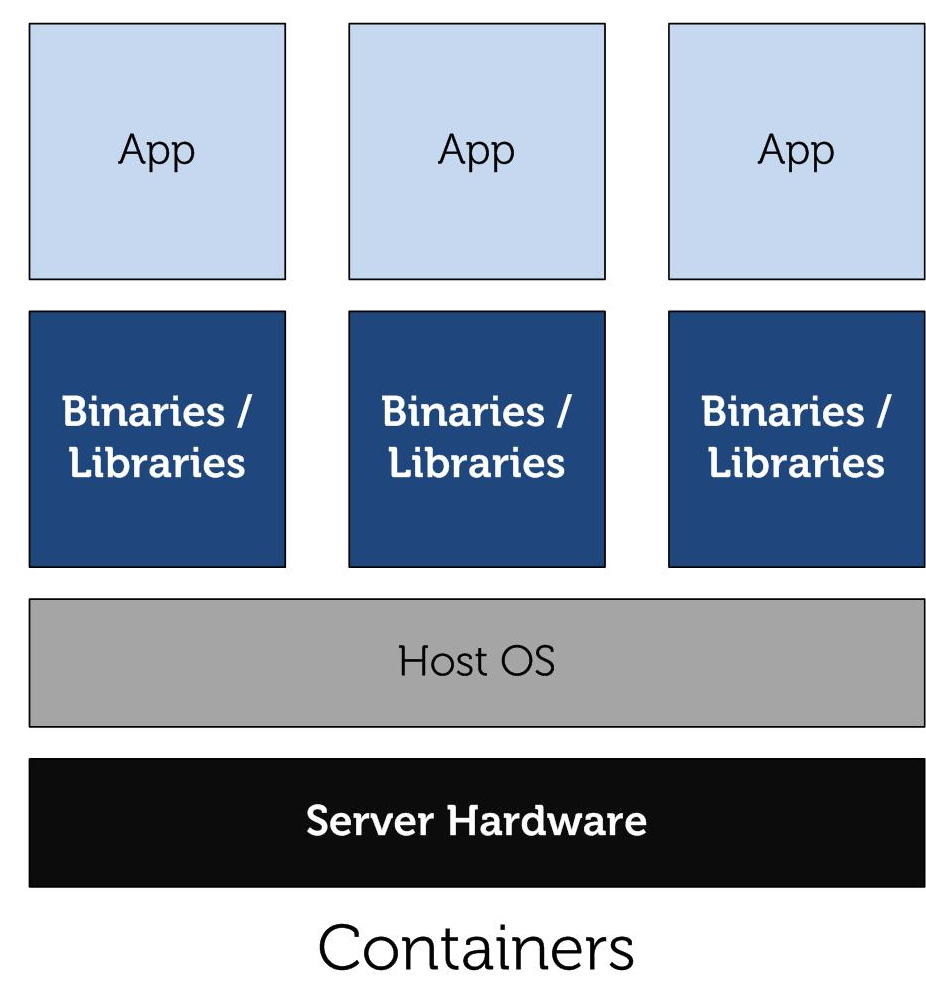
\includegraphics[width=0.45\textwidth]{Figures/containers.png}
    	\caption[Virtualización basada en contenedores]{Virtualización basada en contenedores: los contenedores comparten el sistema operativo del host y por lo tanto no necesitan una copia.}
    	\label{fig:contenedor-arch}
     \end{subfigure}
    ~ 
    \begin{subfigure}[b]{0.48\textwidth}
         \centering
    	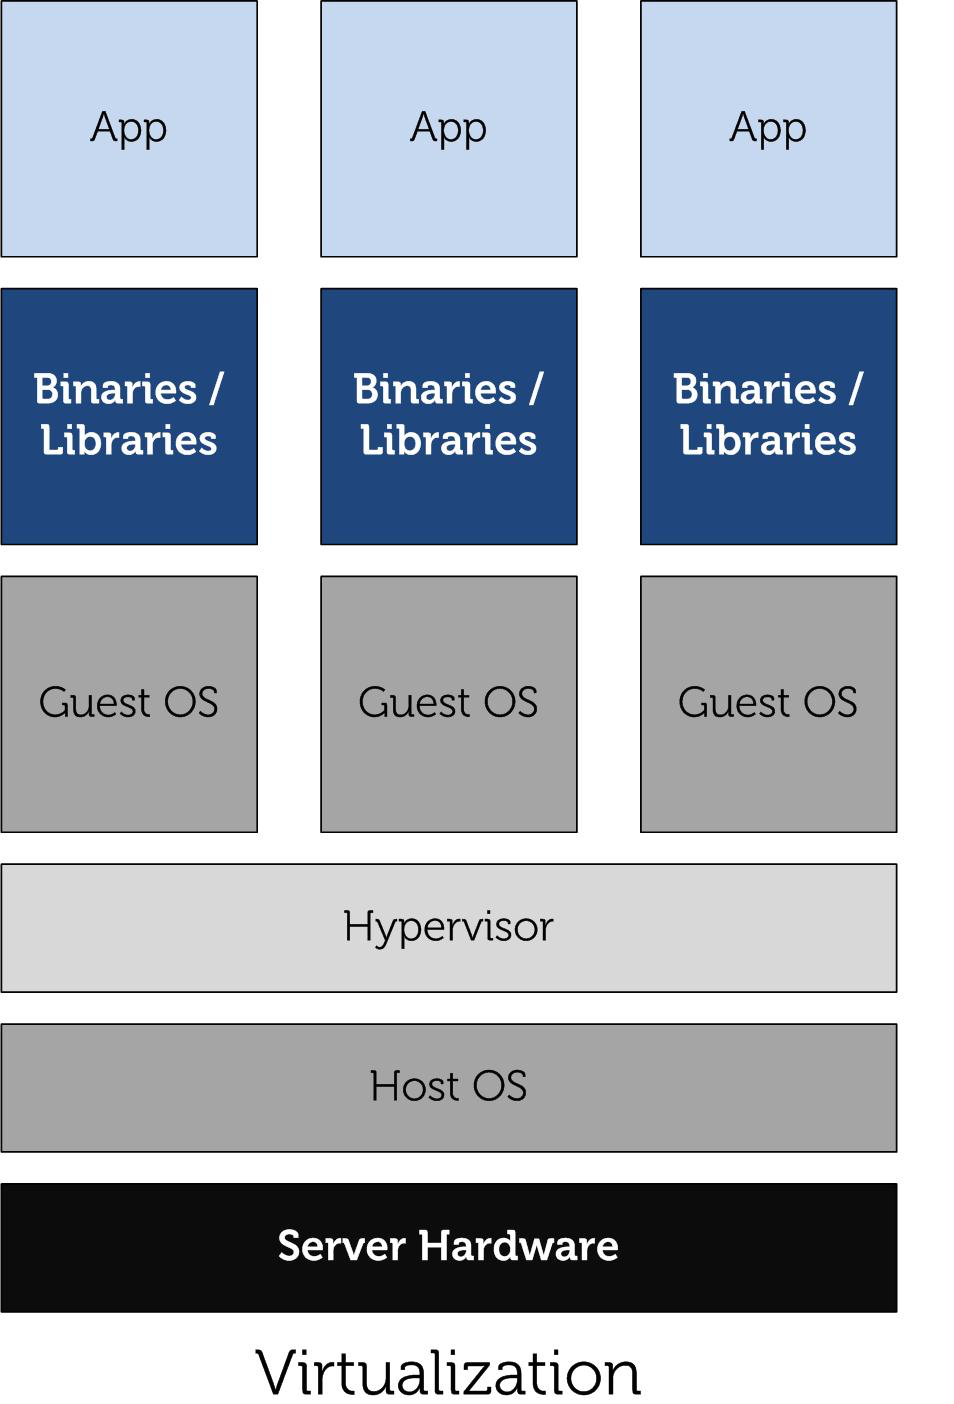
\includegraphics[width=0.45\textwidth]{Figures/virtual.png}
    	\caption[Virtualización basada en máquinas virtuales]{Virtualización basada en máquinas virtuales: las máquinas virtuales requieren un sistema operativo para cada uno.}
    	\label{fig:vm-arch}
     \end{subfigure}
        \caption[Comparación entre virtualizacion basada de contenedores y máquinas virtuales]{Dado que un contenedor comparte recursos, esto reduce significativamente el uso de almacenamiento en comparación a las máquinas virtuales.}
        \label{fig:virtualization}
\end{figure*}

Las diferencias entre la virtualización basada en contenedores y máquinas virtuales presentan características interesantes para la ejecución de aplicaciones y workflows. Dado que un contenedor comparte recursos con el sistema operativo, como las bibliotecas, esto reduce significativamente la necesidad de reproducir el código del sistema operativo, y significa que un servidor puede ejecutar varios ambientes con una sola instalación del sistema operativo. 
Por lo tanto, los contenedores son excepcionalmente ligeros: sólo tienen un tamaño de mega-bytes y sólo tardan unos segundos en arrancar. En comparación con los contenedores, las máquinas virtuales tardan minutos en funcionar y son un orden de magnitud mayor que un contenedor equivalente. \cite{padala2007performance,regola2010recommendations,felter2014updated}. A partir de esto nace la motivación de la utilización de contenedores con una alternativa para alcanzar la conservación física de los ambientes.
Docker es un proyecto open-source que utiliza la tecnología de los contenedores (libcontenedor) para ``construir, migrar y correr aplicaciones distribuidas". Actualmente utilizado por Yelp, Spotify, entre otros \cite{marmolnetworking}
Docker es una solución que simplifica el uso de los contenedores que han estado presente durante más de una década. Primero provee una interfaz simple y segura para crear y controlar contenedores \cite{bui2015analysis}, segundo permite a los desarrolladores empaquetar y correr sus aplicaciones de manera sencilla y además se integra con herramientas terceras que permiten administración y despliegue como Puppet\footnote{\url{https://puppet.com}}, Ansible \footnote{\url{https://ansible.com}} y Vagrant\footnote{\url{https://vagrant.com}}. Y diversas herramientas de orquestación como Mesos \footnote{\url{http://mesos.apache.org/}}, 
Shipyard \footnote{\url{https://shipyard-project.com/}},
Kubernetes \footnote{\url{https://kubernetes.io/}},
RancherOS \footnote{\url{http://rancher.com/rancher-os/}} y 
Docker Swarm \footnote{\url{https://docs.docker.com/swarm/}}.

Docker puede separarse en dos grandes componentes Docker Engine y Client.
Docker Engine es una herramienta liviana y portable para administrar la virtualización. Y Docker Client, provee una interfaz para interactuar con los contenedores con los usuarios a través de RESTful APIs\cite{bui2015analysis}.

\begin{figure}[t]
  \centering
  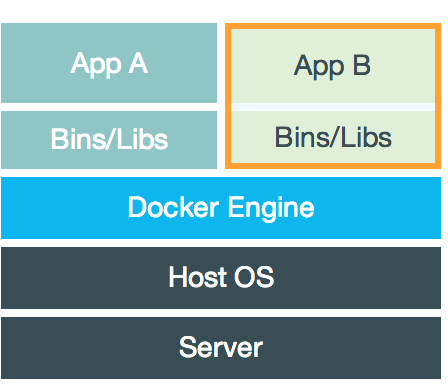
\includegraphics[width=0.3\textwidth]{Figures/docker.png}
    \caption{Arquitectura de Docker}
    \label{fig:docker}
\end{figure}

Docker utiliza una arquitectura de cliente-servidor, \emph{Docker Client} interactúa con \emph{Docker Daemon} y éste construye, maneja y corre los contenedores. Docker Client y Docker Daemon pueden correr en el mismo host o se puede conectar el cliente desde un host remoto. El cliente y el Daemon se comunican en forma de sockets o RESTful API \footnote{\url{https://docs.docker.com/introduction/understanding-docker/}}. 
Una imagen de Docker (\textit{Docker Image}) es una plantilla de solo lectura. Por ejemplo, una imagen puede contener las herramientas básicas de Ubuntu con Apache y una aplicación web instalada o simplemente el sistema operativo. Las imágenes son usadas para construir los contenedores. Y cuando el usuario crea cambios en el contenedor, este cambio no se realiza en la imagen, sino  que Docker añade una capa adicional con los cambios de la imagen\cite{bui2015analysis}. Por ejemplo, si el usuario utiliza una imagen base de Debian, luego añade el paquete emacs y luego añade el paquete apache, el estado de capas estaría representado por la figura \ref{fig:arquitectura}. Esto permite tener un proceso de distribución de imágenes más eficiente dado que solo es necesario distribuir las actualizaciones \cite{bui2015analysis}. El sistema de archivos descrito anteriormente se denomina una sistema de archivo basado en capas.
\begin{figure}[t]
  \centering
  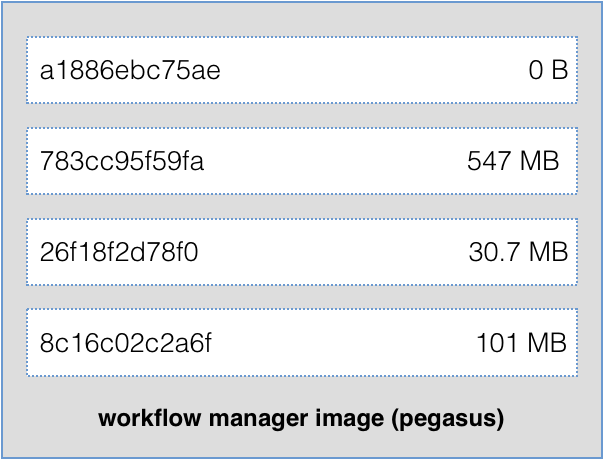
\includegraphics[width=0.6\textwidth]{Figures/docker-filesystems-multilayer}
    \caption[Capas de una imagen de Docker]{Las imágenes Docker con compuestas por capas. 
    La última capa (a1886ebc75ae) es la única capa en modo escritura.}
    \label{fig:arquitectura}
\end{figure}	

Docker Hub es un repositorio que almacena dos tipos de repositorios oficiales y comunitarios. Los repositorios oficiales contienen imágenes públicas y verificadas de empresas y proveedores de software de renombre, como Canonical, Nginx, Red Hat y el propio Docker. Al mismo tiempo, los repositorios comunitarios pueden ser repositorios públicos o privados creados por usuarios y organizaciones individuales, que comparten sus aplicaciones y resultados. 

Usando ese repositorio y una línea de comandos, es posible descargar e implementar imágenes Docker localmente, ejecutando el contenedor en un entorno host, y ejecutando así el software dentro de la imagen. Los usuarios pueden crear y almacenar imágenes en el registro del Docker Hub, creando un archivo descriptor llamado Dockerfile o ampliando uno existente.  Este archivo describe cuáles son los comandos para construido la imagen y por lo tanto los paquetes de software que estarán dentro de la imagen, luego se construye la imagen y finalmente se sube al Docker Hub. Sin embargo, Docker Hub no controla qué paquetes hay en las imágenes, si la imagen se desplegará correctamente o si las imágenes pueden tener algún problema de seguridad. 
Así, las imágenes Docker funcionan como una caja negra, lo que significa que los usuarios saben sólo paquetes principales que se ejecutan dentro del contenedor pero no conocen los otros paquetes necesarios para ejecutarlo.
Hay dos maneras de subir imágenes a un repositorio de usuario, ya sea enviar la imagen desde un host local o automatizando ese proceso desde un repositorio Github \footnote{\url{https://github.com/}}. Para enviar una imagen al Docker Hub, los usuarios necesitan nombrar sus imágenes locales usando su nombre de usuario Docker Hub, y el nombre del repositorio que han creado. 
Después, los usuarios añaden múltiples versiones a un repositorio añadiéndole la versión \texttt{:<tag>}. 
Esta es toda la información que normalmente tienen las imágenes Docker en DockerHub, siendo por tanto casi imposible reproducir el entorno de ejecución si se modifica alguno de los paquetes de software utilizados dentro de las imágenes. 
 
DockerHub permite a las comunidades científicas almacenar y compartir, conservando el contenido de los contenedores, así como comprobar la identidad del editor y recuperar los contenedores de interés. Sin embargo, la información del contenido de cada repositorio no siempre es accesible de forma clara. 
Como la mayoría de las veces sólo se proporcionan descripciones cortas de los contenedores, no es fácil para el usuario entender qué componentes están instalados en ellos. 
Incluso cuando los archivos Dockerfile están disponibles, no son lo suficientemente intuitivos de entender cuáles paquetes están siendo desplegados por cada comando.
%todo: propuesta está aca.
Además, es posible que en el contenedor existan algunos componentes que no estén especificados por el propio Dockerfile. Para abordar este problema proponemos un enfoque automático para analizar el contenido de un contenedor Docker y extraer la información sobre los componentes de software instalados en él. Esta información se convierte en datos semánticos, codificados como RDF bajo el conjunto de ontologías.

Los contenedores Docker consiste de un ambiente virtual: con archivos de usuarios y metadatos, cada contenedor es construido a partir de una imagen base como se mencionó anteriormente. 
Esta imagen indica la base del contenedor y se asocia un proceso inicial, él cual debe correr cuando el contenedor es iniciado.

La figura \ref{lst:simple-docker}describe los pasos incluidos en la creación de un contenedor.

\begin{figure*}
	\begin{lstlisting}[caption={Ejemplo de la ejecución de un contenedor utilizando la imagen Docker},label={lst:simple-docker},language=bash]
	docker run -i -t ubuntu /bin/bash
\end{lstlisting}
\end{figure*}

	\begin{itemize}
		\item \emph{Docker Client} le informa al Docker que debe correr un contenedor.
		\item En este caso el comando \texttt{/bin/bash} será el proceso \texttt{init} o 0 del contenedor
		\item Docker verifica la existencia de la imagen Ubuntu y sino existe en el host, entonces Docker descarga desde el repositorio ya sea privado o publico. Si la imagen existe entonces crea el contenedor.
		\item Asignar el sistema de archivos y montar la capa de escritura, para crear el contenedor debe realizarse en el sistema de archivos y añadir una capa en modo escritura en la imagen.
		\item Crea la interfaz de red que permite que contenedor pueda enviar y recibir paquetes con el host a través del puente (docker0).
		\item Asigna una dirección IP del conjunto de dirección IP disponibles al contenedor
		\item Dependiendo de la configuración de contenedor, Docker enviará a los registros de errores hacia el mismo servidor u otro externo.
	\end{itemize}

Para crear los ambientes virtuales Docker utiliza dos funcionalidades de Linux: \emph{namespaces}\footnote{\url{http://man7.org/linux/man-pages/man7/namespaces.7.html}} y \emph{cgroups}\footnote{\url{http://man7.org/linux/man-pages/man7/cgroups.7.html}}. \emph{cgroups} o \emph{control groups} proveen un mecanismo de contabilidad y limites de recursos que pueden utilizar los contenedores\cite{bui2015analysis}. Los \emph{namespaces} proveen del aislamiento para el contenedor. 
Cuando se crea un contenedor, Docker crea un conjunto de \emph{namespaces} para el contenedor. Los \emph{namespaces} utilizados por Docker son: mount (mnt) para el manejo del montaje, PID para el aislamiento de los procesos, net para el manejo de interfaces y IPC para acceder a recursos de IPC. 
Docker logra el aislamiento de los procesos separando los procesos en \emph{PID namespaces}.
\emph{PID namespaces} (añadido en el kernel \( \geq 2.6.3.2)\) logdando que un proceso que se encuentra en el contenedor solo pueda ver procesos que se encuentra en ese contenedor. Por lo tanto un atacante no puede observar procesos de otro contenedor, lo que aísla al contenedor este nivel \cite{bui2015analysis}.
Docker usa \emph{mount namespaces} o \emph{filesystem namespaces} para aislar los \emph{filesystems} asociados a los contenedores. De la misma forma que ocurre con los procesos, los eventos del sistema de archivos que ocurre en el contenedor sólo afectan a ese contenedor.

Cómo se menciono anteriormente, Docker utiliza \emph{cgroups} que permite especificar que \emph{device} puede ser utilizado con el contenedor. Esto bloquea la posibilidad de crear y usar \emph{device nodes} que puedan ser utilizados para atacar el host. Los \emph{device nodes} que son creados para cada contenedor por defecto: son: /dev/console, /dev/null, /dev/zero, /dev/full, /dev/tty*, /dev/urandom, /dev/random, /dev/fuse.
IPC (\emph{inter-process communication} es un conjunto de objetos para el intercambio de datos a través de los procesos, como semáforos, colas de mensajes, segmentos de memoria compartida. Los procesos corriendo en los contenedores utilizan \emph{IPC namespaces} que permite la creación de un \emph{IPC} separado y independiente para cada contenedor, con esto se previene que procesos en un contenedor interfieran con otros contenedores o el host.
Para cada contenedor, Docker crea una red independiente usando \emph{network namespaces}, compuesta de su propia IP, rutas, \emph{network devices}. Esto permite que el contenedor pueda interactuar con otro host a través de su propia interfaz.
Por omisión, la conexión se realiza gracias al host que provee un \emph{Virtual Ethernet bridge} en la máquina host, llamado docker0 que automáticamente realiza un \emph{forward} de los paquetes entre las interfaces. Cuando Docker crea un nuevo contenedor, se crea una interfaz de red virtual con un nombre único que se conecta con el \emph{bridge (docker0)} y con la interfaz \emph{eth0} del contenedor \cite{bui2015analysis}.
Además \emph{Cgroups} controla la cantidad de recursos como CPU, memoria, \emph{disk I/O} que el contenedor puede utilizar. 
Fijando estos parámetros se puede limitar los efectos de un dtaque de denegación de servicio (DDoS).

\section{Clair}\label{sec:clair}

Clair~\footnote{https://github.com/coreos/clair/} es un proyecto de código abierto para el análisis estático de vulnerabilidades en contenedores de aplicaciones (actualmente incluyendo appc \footnote{\url{https://coreos.com/rkt/docs/latest/app-container.html}} y Docker).
   
En intervalos regulares, Clair ingiere metadatos de vulnerabilidades un conjunto configurado de fuentes y los almacena en la base de datos. 
Para analizar las imágenes, los clientes utilizan la API de Clair y el sistema indexa sus imágenes; esto crea una lista de características presentes en la imagen y las almacena en la base de datos.

Clair define su propia terminología:

\begin{description}
	\item [Feature:] cualquier funcionalidad que éste presente en el sistema de archivos que sea una indicación de una vulnerabilidad (e.g. presencia de un archivo o paquete)
	\item [Feature Namespace:] contexto de \emph{feature} o vulnerabilidades (e.g. un sistema operativo o lenguaje)
	\item [Vulnerability Source (vulnsr):] el componente de Clair que rastrea los datos de vulnerabilidad y los importa a la base de datos de Clair
	\item [Vulnerability Metadata Source (vulnmdsrc):] el componente de Clair rastrea los metadatos de vulnerabilidad y los asocia con las vulnerabilidades en la base de datos de Clair
\end{description}

Clair se compone de distintos controladores (\emph{drivers}).

\begin{description}
	\item [featurefmt:] identifica el formato de las funcionalidades de una capa (e.g. apt).
	\item [featurens:] identifica cuáles son los \emph{namespaces} que son aplicables a la capa (e.g. ubuntu 16.04).
	\item [imagefmt:] determina la ubicación del sistema de archivos raíz de la capa (e.g. Docker).
	\item [versionfmt:] determina y compara los strings de la versión (e.g. rpm).
	\item [vulnmdsrc:] descarga los metadatos de las vulnerabilidades para ser procesados (e.g. National vulnerability database - NVD \footnote{\url{https://nvd.nist.gov/}} ) .
	\item [vulnsrc:] descarga las vulnerabilidades para un conjunto de \emph{namespaces} (e.g. \emph{Alpine Security Database of Backported fixes})
\end{description}

La figura \ref{table:clair-datasources} muestra los drivers implementados por Clair.

\begin{table}[t]
\begin{tabular}{|l|l|l|l|}
\hline
Fuente de datos             & Datos recolectados                                                                                                          & Formato & Licencia \\ \hline
Debian Security Bug Tracker & \emph{Namespaces:} Debian 6, 7, 8 y inestable                                                                               & dpkg    & Debian   \\ \hline
Ubuntu CVE Tracker          & \begin{tabular}[c]{@{}l@{}}\emph{Namespaces:} Ubuntu 12.04, 12.10,\\  13.04, 14.04, 14.10, 15.04, 15.10, 16.04\end{tabular} & dpkg    & GPLv2    \\ \hline
Red Hat Security Data       & \emph{Namespaces:} CentOS 5, 6, 7                                                                                           & rpm     & CVRF     \\ \hline
Oracle Linux Security Data  & \emph{Namespaces:} Oracle Linux 5, 6, 7                                                                                     & rpm     & CVRF     \\ \hline
Alpine SecDB                & \begin{tabular}[c]{@{}l@{}}\emph{Namespaces:} Alpine 3.3, Alpine 3.4, \\ \\ Alpine 3.5\end{tabular}                         & apk     & MIT      \\ \hline
NIST NVD                    & Metadatos genéricos de vulnerabilidades                                                                                     & N/A     & Pública   \\ \hline
\end{tabular}
\caption{Fuente de datos implementadas por Clair}
\label{table:clair-datasources}
\end{table}

\section{Sistemas de paquetes}

Un gestor de paquetes es un conjunto de herramientas de software qué automatiza el proceso de instalación, actualización, configuración y eliminación de programas para el sistema operativo de un ordenador de forma coherente.

Un gestor de paquetes se ocupa de paquetes, distribuciones de software y datos en ficheros de archivo. Los paquetes contienen metadatos, como el nombre del software, la descripción de su propósito, el número de versión, el proveedor, la suma de comprobación y una lista de dependencias necesarias para que el software funcione correctamente. 

Tras la instalación, los metadatos se almacenan en una base de datos de paquetes local. Esta base de datos se guarda en un archivo en el sistema de archivos. Por lo tanto, la información de los componentes del software de una imagen se encuentra en cada una de sus capas.
Dependiendo del sistema de paquetes, se puede utilizar otras herramientas para obtener mayor información utilizando la información que se encuentra en la base de datos.

A continuación se describe los sistemas de paquetes populares

\subsection{rpm}\label{sub:rpm}
\emph{RPM Package Manager} (RPM) es un sistema de empaquetado abierto, que se ejecuta en Red Hat Enterprise Linux así como en otros sistemas Linux y UNIX.
El archivo de base de datos de rpm se encuentra ubicado en \verb|/var/lib/rpm/Packages|. La información disponible en ese archivo es: Nombre, Versión, Lanzamiento, Arquitectura, Fecha de instalación, Grupo, Tamaño, Licencia, Firma, RPM de origen, Fecha de construcción,  Host de reconstrucción, Proveedor del paquete, URL, Resumen y  Descripción.
\subsection{dpkg}\label{sub:dpkg}

Debian Package Manager (dpkg) es un sistema de gestión de paquetes en el sistema operativo libre Debian y sus numerosos derivados. dpkg se utiliza para instalar, eliminar y proporcionar información sobre los paquetes .deb. 

El archivo de base de datos de dpkg se encuentra ubicado en \verb|/var/lib/dpkg/status| utilizando formato texto plano.  La información disponible es: Paquete, Estado, Prioridad, Sección, Tamaño de la instalación, Encargado del mantenimiento, Arquitectura, Fuente, Versión, Reemplaza a otro paquete, Dependencias y Recomendaciones.

\subsection{apk}\label{sub:apk}

apk es un sistema de gestión de paquetes en el sistema operativo Alpine. Alpine se ha convertido una distribución de Linux muy utilizada en contenedores debido a que la imagen tiene un tamaño menor a los 10 MB.
El archivo de base de datos de apk se encuentra ubicado en \verb|/lib/installed|. La información disponible se basa la especificación de apk \footnote{\url{https://wiki.alpinelinux.org/wiki/Apk_spec}}: Arquitectura, Suma del pull, Dependencias, Ruta de archivos, Tamaño, Licencia, Nombre del paquete, Descripción, URL, git commit del paquetes, tiempo de construcción, entre otros. 

\subsection{Conda}\label{sub:conda}
Conda es un gestor de paquetes, dependencias y entornos para lenguajes Python, R, Ruby, Lua, Scala, Java, JavaScript, C/ C++, FORTRAN y que es ampliamente utilizado en entornos de \textit{Jupyter notebook}.

El archivo de base de datos de Conda se encuentra ubicado en \verb|conda/history| según la posición del ambiente. La información disponible se basa la especificación de Conda \footnote{\url{https://conda.io/docs/user-guide/tasks/build-packages/package-spec.html}}: Nombre, versión, versión de construcción, número de construcción, dependencias, arquitectura, plataforma y archivos.

\section{Web Semántica}

La web semántica es un extensión \emph{World Wide Web} añadiendo un conjunto de estándares diseñado por la \emph{World Wide Web Consortium} con el objetivo de la creación de tecnologías para publicar datos legibles por aplicaciones informáticas. 
Para lo lograr lo anterior, se añaden metadatos semánticos y ontologías para describir el contenido y generar relaciones entre los datos, esta representación se realiza de una manera formal.
Consecuentemente, la información disponible pueden ser procesadas de manera automática mejorando la inter operatividad entre distintos sistemas informáticos que realizan búsquedas sin operadores humanos.
El término fue acuñado por Tim Berners-Lee y describe una red de datos que puede ser procesada por máquinas. Además, en \cite{berners1992world} se afirma la necesidad de que los datos se transformen desde objetos legible por personas a información semántica diseñada para las máquinas.
Es por ello que la web semántica ha definido diversos estándares para construir una descripción formal de los conceptos, términos y relaciones. Estos estándares definidos por W3C incluyen: RDF, RDFS, SPARQL, Notation3 (N3), N-Triples, Turtle y OWL.

\subsection{RDF}\label{sw:rdf}
RDF (del inglés \emph{Resource Description Framework}) es un modelo estándar para el intercambio de datos en la Web. 
Distintas especificaciones se han publicado: en 1999 se adopto como una recomendación del W3C y las especificaciones 1.0 y 1.1 se publicaron en 2004 y 2014 respectivamente \cite{bikakis2013semantic}.

RDF extiende la estructura de enlace de la Web para usar URIs para nombrar la relación entre cosas. Un triple tiene la forma de expresión  $\langle sujeto, predicado, objeto \rangle$. Donde el $sujeto$ indica el recurso, el $predicado$ nombra la relación entre el $sujeto$ y $el objeto$

%todo: rewrite
\subsection{RDFS}
RDFS (de las siglas del inglés \emph{Resource Description Framework Schema},
también llamado RDF Schema) es un vocabulario que extiende RDF utilizando un
conjunto de clases y propiedades que mejoran la creación de modelos como son:
\tt{Class} para declarar clases, \tt{subClassOf} para denotar herencia,
\tt{range} y \tt{domain} para el rango y dominio de cierta propiedad
(\tt{rdf:Property}), entre otras.

En 1998 se presento y fue introducido como recomendación del W3C en 2004
\cite{bikakis2013semantic}.

\subsection{OWL}

OWL (del inglés \emph{Web Ontology Language}) es un lenguaje semántico para publicar y compartir ontologías complejas en la W3C, OWL se desarrolla como una extensión de vocabulario de RDF (Resource Description Framework). 
Se han publicados versiones de OWL. La primera OWL publicada el 2004 y la segunda version ``OWL 2'' fue publicada el 2009 como una revisión y extensión de la versión inicial Usualmente cuando se habla de ``OWL'' se refiere a la versión a la versión del 2004.
